\chapter{نبذه عن لغة بايثون}
\noindent
أعتقد انه من الاهمية بمكان ان يتعلم كل واحد منا لغة البرمجة وذلك لانها  تساعدنا على تعلم طريقة التفكير الصحيحة
\begin{flushright} 
ستيفن جوبز
\end{flushright}
\rule{\textwidth}{1pt}
\section{تعريف لغة بايثون }
بايثون لغة برمجية مفتوحة المصدرسهلة التعلم يمكن الاعتماد عليها في كتابة الكثير من التطبيقات البرمجية القوية. واكبر دليل على ذلك هو استخدام وكالة الارصاد الامريكية ناسا وشركة قوقل وياهو وغيرها من الشركات الكبرى لهذه اللغة في بناء برامجهم المختلفة. 
\section{نشئة لغة بايثون}

كانت بدايات نشئة هذه اللغة في هولندا على يد شخص يدعي جويدو فان روزم
\textenglish{(Guido van Rossum)}
 في نهاية الثمانيات الميلادية من القرن العشرين. لكن لم يتم الاعلان عنها الا في عام ١٩٩١م.   ويعتبر فتح مصدر هذه اللغة من اهم الاسباب التي ادت الى زيادة شهرتها وذلك من خلال تكوين مجتمع برمجي نشط حولها اسهم في  انشاء مكتبات كثيرة سهلت على المطورين الاخرين بناء تطبيقاتهم بسرعة و سهوله فائقة مقارنة باللغات البرمجية الاخري.

\section{ مزايا لغة بايثون}
للغة بايثون مزايا عدة جعلت منها اللغة المفضلة الاولى لدى كثير من المبرمجين ومن بين اهم هذه المزايا نذكر:
\begin{enumerate}
\item
سهولة تراكيبها اللغوية: فاكوادها البرمجية تكتب بطريقة قريبة جدا من اللغة الانجليزية. لذلك نجدها لاتشكل اي عائق امام أي مبرمج ان يفهم الأكواد المكتبوبة من قبل مبرمجين اخرين عندما يستدعي الامر صيانة تلك الاكواد اوتحديثها.
\item
المرونة: يمكن تشغيل وتطوير البرامج المكتوبة بلغة بايثون على معظم انظمة التشغيل المعروفة. فالأكواد التي تم تطويرها على نظام ويندوز يمكن تشغيلها على نظام ماك ولينكس والعكس صحيح دون الحاجة الى اعادة بناء الأكواد
 .(compiling)
\item
كثرة المكتبات: يعتبر توفر المكتبات من اهم المزايا التي تقدمها اللغة للمبرمجين لتزيد من فعاليتهم في بناء التطبيقات. لذلك عند تنصيب اصدارة بايثون نجد انها تحتوي على مكتبات قياسية كثيرة بعضها يعتبر جزء لا يتجزء من تراكيب اللغة كمكتبة الارقام والقوائم وبعضها الاخر يعمل على تسهيل التعامل مع انظمة التشغيل اما الجزء الاكبر من هذه المكتبات فهو اختياري يتم استيراده متى ما دعت الحاجة لذلك. كما ان هناك مكتبات اخري تحتاج الى تنصيب قبل ان يتمكن المبرمج من استيرادها واستخدامها في برنامجه. وهذه المكتبات مجانية ويمكن تحميلها وتنصيبها اما من الموقع الخاص بالمطورين لهذه المكتبة او من موقع
 \href{http://pypi.python.org}{http://pypi.python.org}
  والذي يحتوي حتى وقت كتابة هذه السطور على 69478 مكتبة مجانية جاهزة يمكن استخدامها في بناء التطبيقات المختلقة.
\item
التكامل مع لغات برمجية اخرى: يمكن استخدام بايثون كلغة مساندة تمكن المستخدم لبرنامج مكتوب بلغة سي (C) او سي بلس بلس (C++) مثلا من زيادة او تعديل خصائص ذلك البرنامج ليتناسب مع احتياج المستخدم. ومن أقرب الامثلة على ذلك هو استخدام لغة بايثون في برنامج فري كاد (FreeCAD) كلغة برمجة نصية لتحكم بكافة خصائص البرنامج ووظائفه.
\end{enumerate}

\section{اصدارت بايثون}
هناك اصدارتان لبايثون. الإصدارة الأولى تعرف ببايثون 2 وهي الاقدم والاصدارة الاخرى تدعى بايثون 3 وهي الاحدث.
\section{تنصيب مفسر لغة بايثون}
\subsection{تنصيب بايثون على نظام ويندوز}

اذا كنت تستخدم اي من انظمة ميكروسوف ويندوز سوا القديم منها او الحديث فانك تحتاج الى تنصيب مفسر لغة بايثون على هذا النظام. واليك الخطوات التالية التي 
تساعدك على عمل ذلك:
\begin{enumerate}
\item
حمل مفسر بايثون من الموقع التالي:
\href{https://www.python.org/downloads/}{http://python.org/downloads/}
يمكنك الاختيار بين احدى الاصدارتين ٢ او ٣. في هذا الكتاب سوف نستخدم الاصدارة ٢. ليس هناك اختلاف جذري بين الاصدارتين في كتابة اكواد اللغة وسوف نشير الى مواضع الاختلاف متى ما تطرقنا الي ذلك عند شرحنا لتراكيب لغة بايثون.
\item
نصب مفسر بايثون باتباع التعليمات الموجودة في برنامج التنصيب
\item
جهز بيئة ويندوز للتعرف على مفسر بايثون باتباع الخطوات التالية:
\end{enumerate}
\subsection{تنصيب بايثون على ابل ماك}
يأتي نظام تشغيل ماك وقد نصب عليه مفسر بايثون ذو الاصادرة رقم ٢. ويمكن التأكد من ذلك باتباع الخطوات التالية:
\begin{enumerate}
\item
قم بتشغيل محرر الاوامر في الماك "terminal" باجدى الطريقتين التاليتين:
\begin{enumerate}
\item
الذهاب الى ملف التطبيقات "Application" من ادارة الملفات "Finder" واختيار محرر الاوامر "terminal" من هناك
\item
الضغط على زر المسافة و زر الاوامر "cmd" في آن واحد تم البحث عن برنامج "terminal"
\end{enumerate}
\item
اكتب في محرر الاوامر الامر التالي بعد علامة الدولار \$ :
 
\begin{figure}[H]
  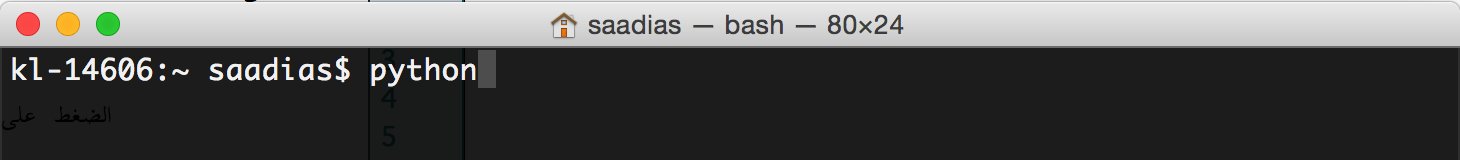
\includegraphics[width=\linewidth]{figures/startpython.png}
  \caption{طريقة بدء مفسر بايثون من محرر الاوامر في الماك}
  \label{fig:startpython}
\end{figure}
بعد الضغط على زر الادخال سوف تحصل على الاتي:

\begin{figure}[H]
  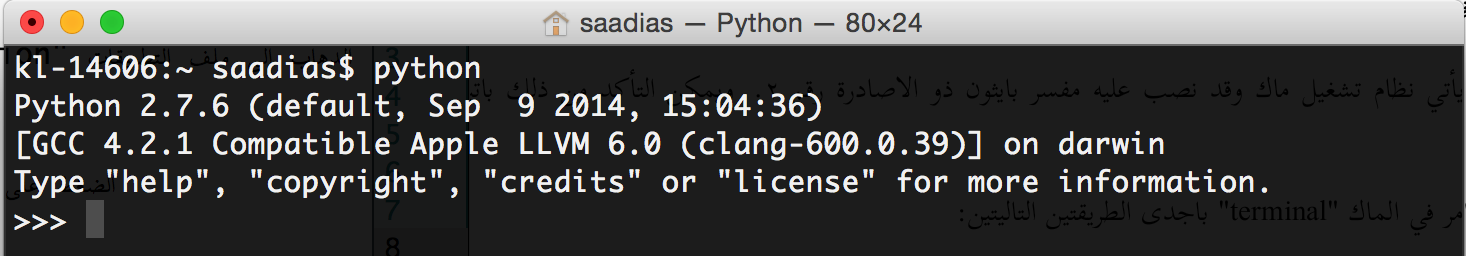
\includegraphics[width=\linewidth]{figures/startpython2.png}
  \caption{بداية تشغيل مفسر اوامر بايثون}
  \label{fig:startpython2}
\end{figure}

وهو يدل على ان بايثون منصب على هذا الجهاز وهو من الاصدارة رقم ٢.٧.٩  كما ان المفسر يبدا مباشرة بالوضع التفاعلي والذي يبدأ بمؤشر خاص 

\end{enumerate}
\subsection{تنصيب بايثون على نظام لينكس (اوبينتو)}
:

كما هو الحال مع نظام ماك فان نظام اوبينتو لينكس يحتوي على مفسر بايثون وهو كذلك من الاصدارة رقم ٢. لتأكد من وجود بايثون على ابيونتو يمكن اتباع نفس الخطوات التي عملنها مع نظام الماك.

\begin{figure}[H]
  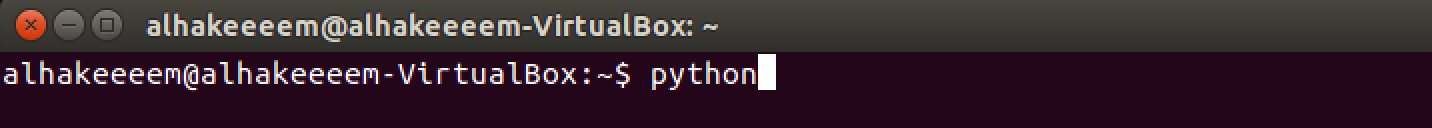
\includegraphics[width=\linewidth]{figures/ubintupython.png}
  \caption{طريقة تشغيل مفسر بايثون في نظام لينكس اوبينتو}
  \label{fig:startpython2}
\end{figure}

\begin{figure}[H]
  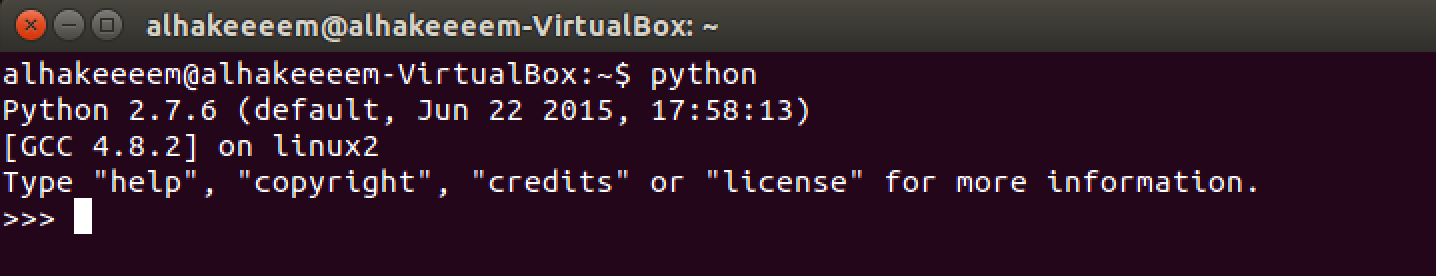
\includegraphics[width=\linewidth]{figures/ubintupython2.png}
  \caption{بدء تشغيل مفسر بايثون في نظام لينكس اوبينتو}
  \label{fig:startpython2}
\end{figure}
هنا ياتي بايثون باصدارة رقم ٢.٧.٦ وكذلك يبدأ بالوضع التفاعلي.		

\section{طريقة كتابة الكود البرمجي في بايثون}
هناك طريقتان يمكن بهما كتابة الاكواد البرمجية لبايثون:
\begin{enumerate}
\item
الطريقة التفاعلية:
وهي الطريقة التي تمكن المستخدم من رؤية نتاتج الامر البرمجي مباشرة بعد الضغط على زر الادخال. وهذه الطريقة تجعل من بايثون اشبه بالالة الحاسبة حيث يتم الحصول على النتائج مباشرة بعد معالجتها من قبل المفسر.لتاكد من ادراكك لهذه الطريقة يمكنك تجربة كتابة الاكود الاتية بعد مؤشر بايثون الخاص وضغظ زر الادخال بعد كل سطر.
\begin{enumerate}
\item

print "welcome to python world"
\item
2+2
\item
x=7
\item
print x
\end{enumerate}
اذا قمت بادخال الاوامر السابقة بشكل صحيح فانك سوف تحصل على النتائج الموضحة في الشكل ادناه:
\begin{figure}[H]
  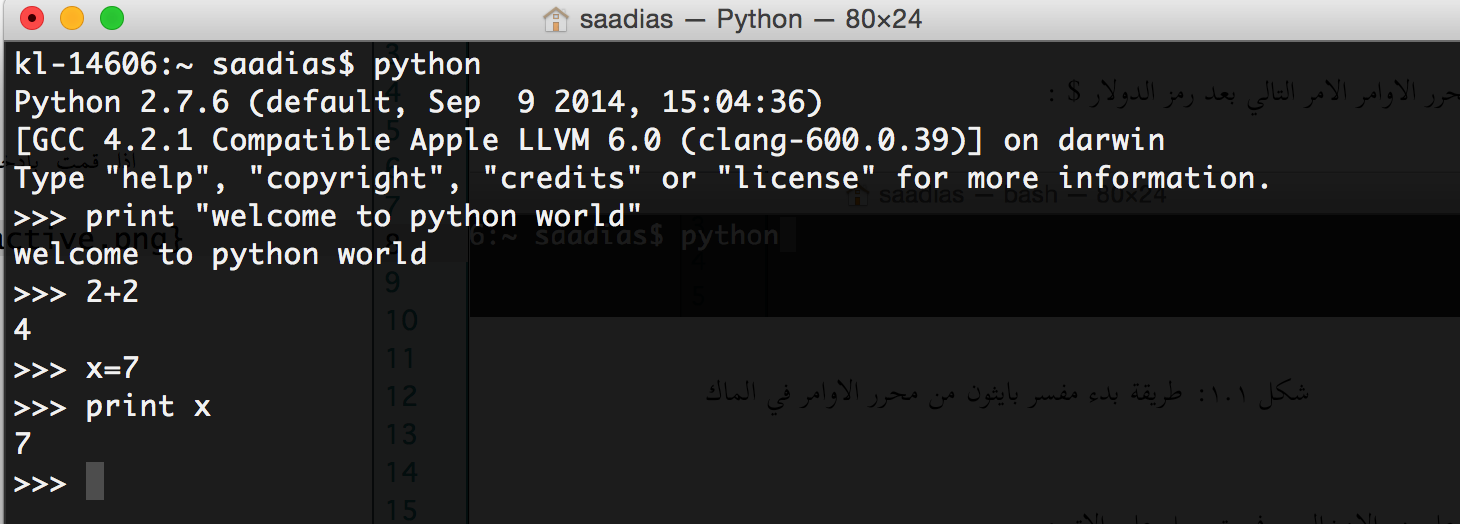
\includegraphics[width=\linewidth]{figures/interactive.png}
  \caption{الوضع التفاعلي لمفسر بايثون}
  \label{fig:startpython2}
\end{figure}
اذا لم تزل غير متاكد من استيعابك لهذه الطريقة يمكنك زيارة موقع الكتاب ومشاهدة الفديو التوضيحي لهذه الطريقة.
\item
استخدام محرر النصوص:
يأتي مع مفسر بايثون محرر نصوص يدعى "ايدل" ويمكن تشغيلة بكاتبة الامر idle من خلال محرر الاوامر في ماك ولينكس. قد يكون idle غير منصب على نظام لينكس اوبينتو لذلك سوف تظهر له تعليمات تبين لك طريقة تنصيبه كما في الشكل التالي:
\begin{figure}[H]
  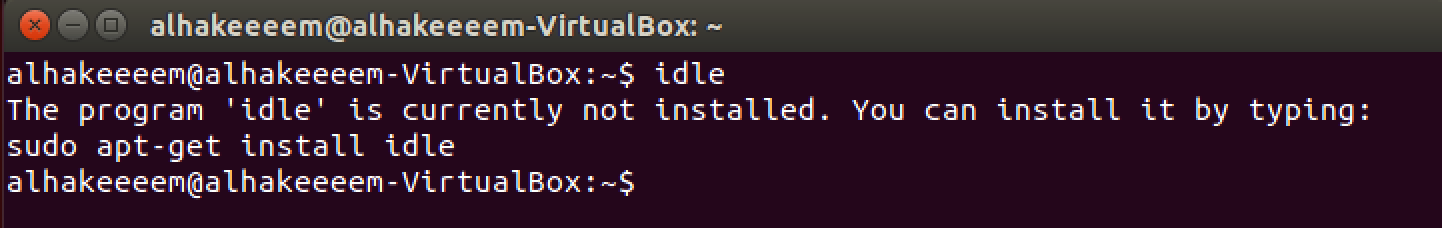
\includegraphics[width=\linewidth]{figures/installidle.png}
  \caption{idle غير منصب على نظام لينكس اوبينتو}
  \label{fig:startpython2}
\end{figure}
ويكمن القيام بعملية التنصيب بادخال الامر التالي في محرر الاوامر:
\begin{flushleft}
sudo apt-get install idle
\end{flushleft}
سوف يطلب منك نظام ادخال كلمة المرور قبل تنفيذ امر التنصيب قم بادخال كلمة المرور الخاصة بك ثم اضغط على زر الادخال. عند اتمام علمية التنصيب ادخل الامر idle لتشغيل محرر النصوص الخاص ببايثون. سوف تظهر له نافذة مستقلة مشابهه لمحرر بايثون التفاعلى السابق انظر الشكل س. حيث يكمنك ان تحصل على نفس النتائج اذا قمت بادخال اومر بايثون انفة الذكر.
\begin{figure}[H]
  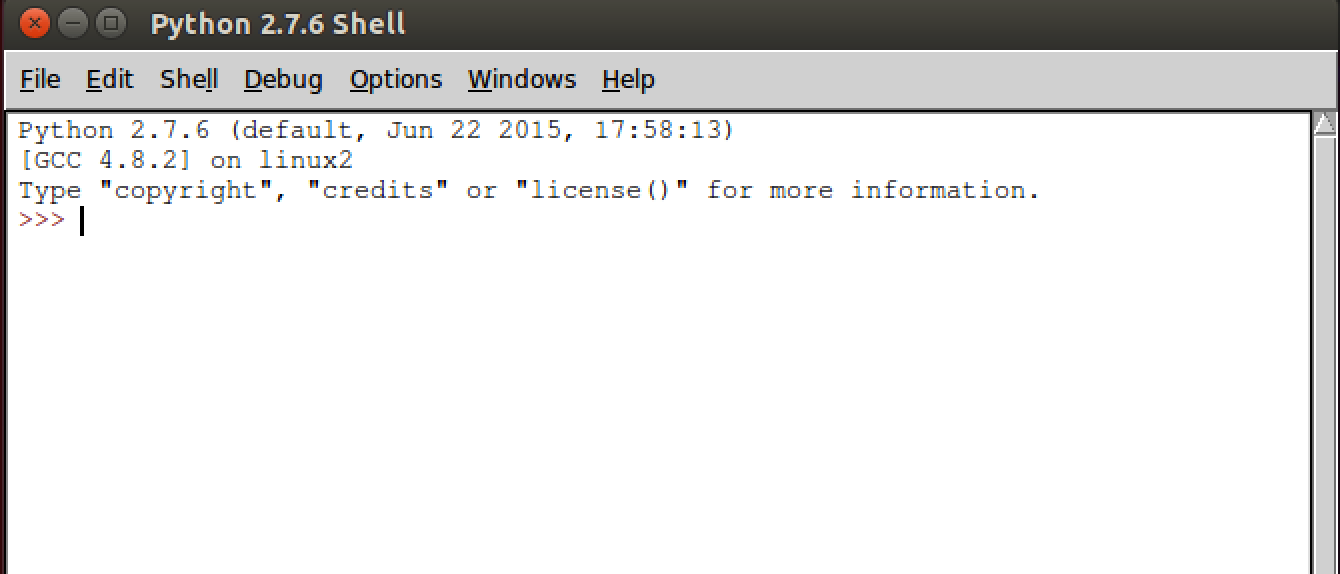
\includegraphics[width=\linewidth]{figures/idle.png}
  \caption{محرر نصوص بايثون}
  \label{fig:startpython2}
\end{figure}
\end{enumerate}